In the following, we describe the detailed implementation of the proposed architecture in Chapter~\ref{sec:architecture}.

\subsection{System wide fine design}\label{subsec:system-wide-design}

\subsubsection{Data Transfer Objects (DTOs)}
The \textit{DTO}s are classes that correspond to the request-bodies and response-bodies as declared in the REST-api. \newline
Due to the fact that these classes will be used in all components, i.e.\ server and client, it makes sense to define these as general as possible.
We used only primitive data types and only properties to ensure compatability across all programming languages. \newline
The simplicity of the DTOs allowsus to use automatic serialization from- and into JSON format.
The \textit{DTO}s are visualized in Figure~\ref{fig:dtos}.

\begin{figure}
    \centering
    \fbox{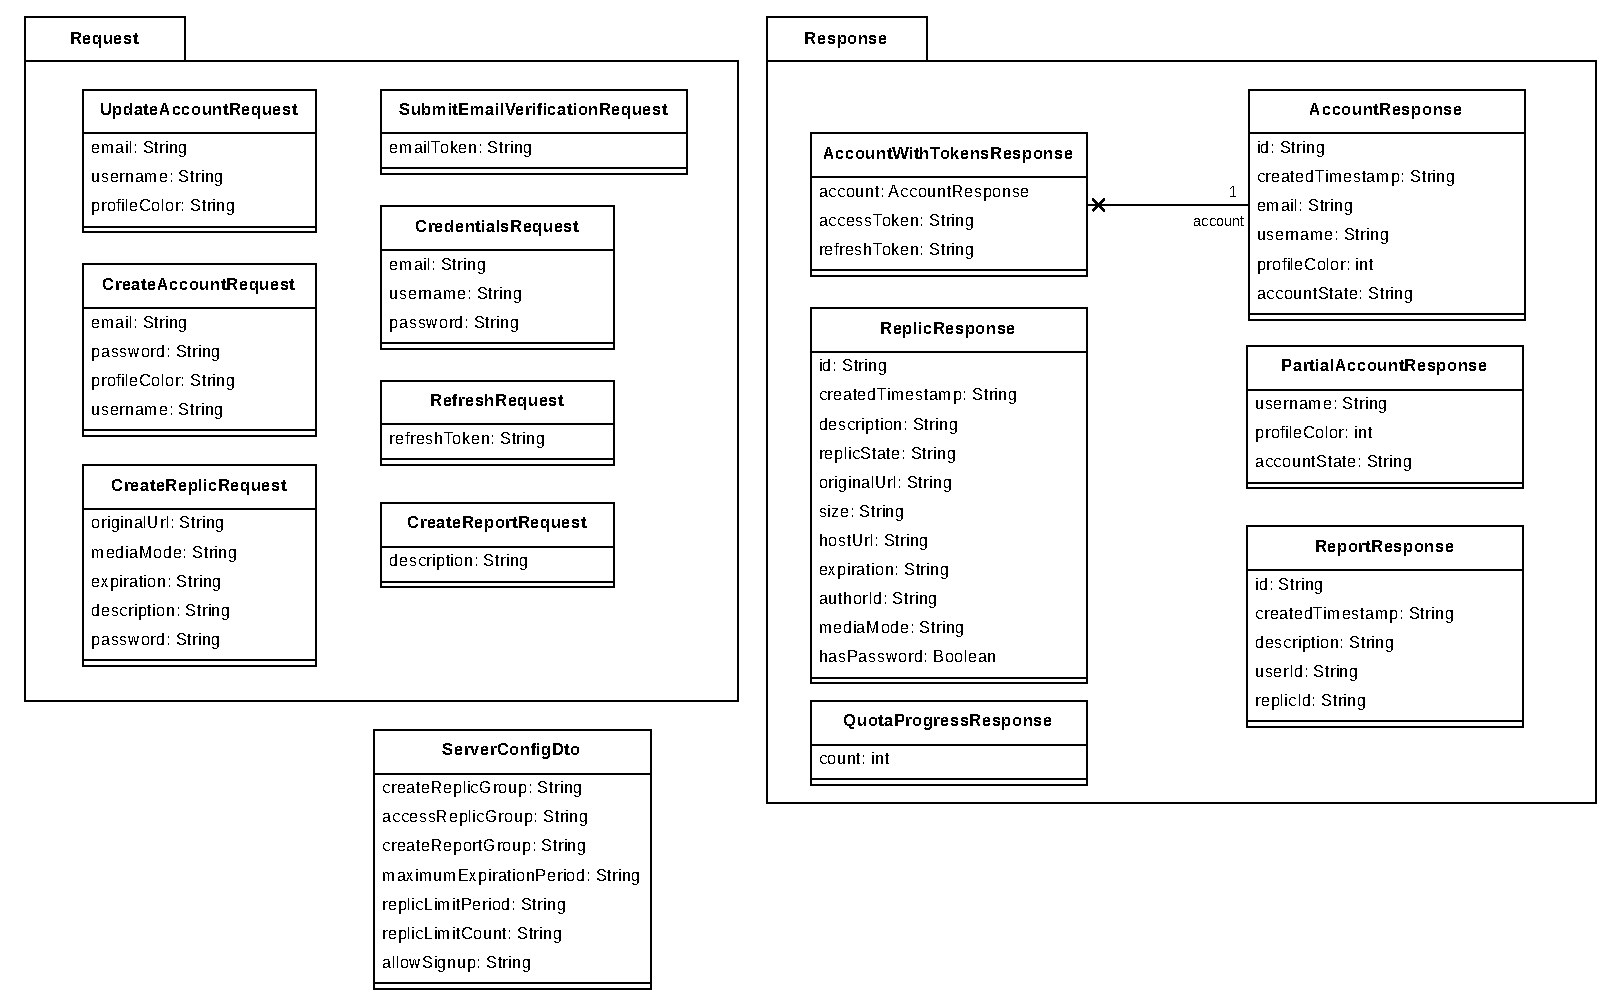
\includegraphics[angle=90,width=\linewidth]{dtos}}

    \caption{Data Transfer Objects}
    \label{fig:dtos}
\end{figure}

\subsubsection{Authentication flow}
Clients will be authenticating themselves with \textit{Json-Web-Tokens} (JWTs) \footnote{https://www.jwt.io/}.

\paragraph{JWTs}
A \textit{JWT} is a string with the following structure: \newline
\begin{center}
    \textit{\textless base64(header)\textgreater.\textless base64(payload)\textgreater.\textless signature\textgreater}
\end{center}

\subparagraph{Header}
The header is a json-object containing the attributes \texttt{alg} ("Algorithm") and \texttt{typ} ("Type of token").
In our case, this header will look like:
\begin{verbatim}
    {
        "alg": "HS256",
        "typ": "jwt"
    }
\end{verbatim}

\subparagraph{Payload}
The payload is a json-object that can contain a selection of attributes.
In our case, the payload will contain the following attributes:
\begin{itemize}
    \item \texttt{iss}: Constant value of \("\)replic-read-server\("\)
    \item \texttt{exp}: ISO-8601 timestamp of the expiration time of the JWT\@.
    \item \texttt{sub}: The id of the account the JWT is created for.
\end{itemize}

\subparagraph{Signature}
The signature is created from the header and payload in the following way: \newline
\begin{center}
    \begin{verbatim}
        HMACSHA256(
        base64(header) + "." +
        base64(payload),
        kessecretret
        )
    \end{verbatim}
\end{center}
where \texttt{secret} is a private key, longer than 256 bits. \newline
Signing the JWT with a private key guarantees the server, that, when presented a JWT by a client, the payload has not been changed.

\paragraph{Logging in}
When a client wants to authenticate, a request with the credentials is sent to \texttt{/auth/login/}.
The server saves a new \textit{refresh-token} and creates a new \textit{JWT} for the client, and returns both these tokens. \newline
Figure~\ref{fig:logging-in} visualizes this flow.

\begin{figure}
    \centering
    \fbox{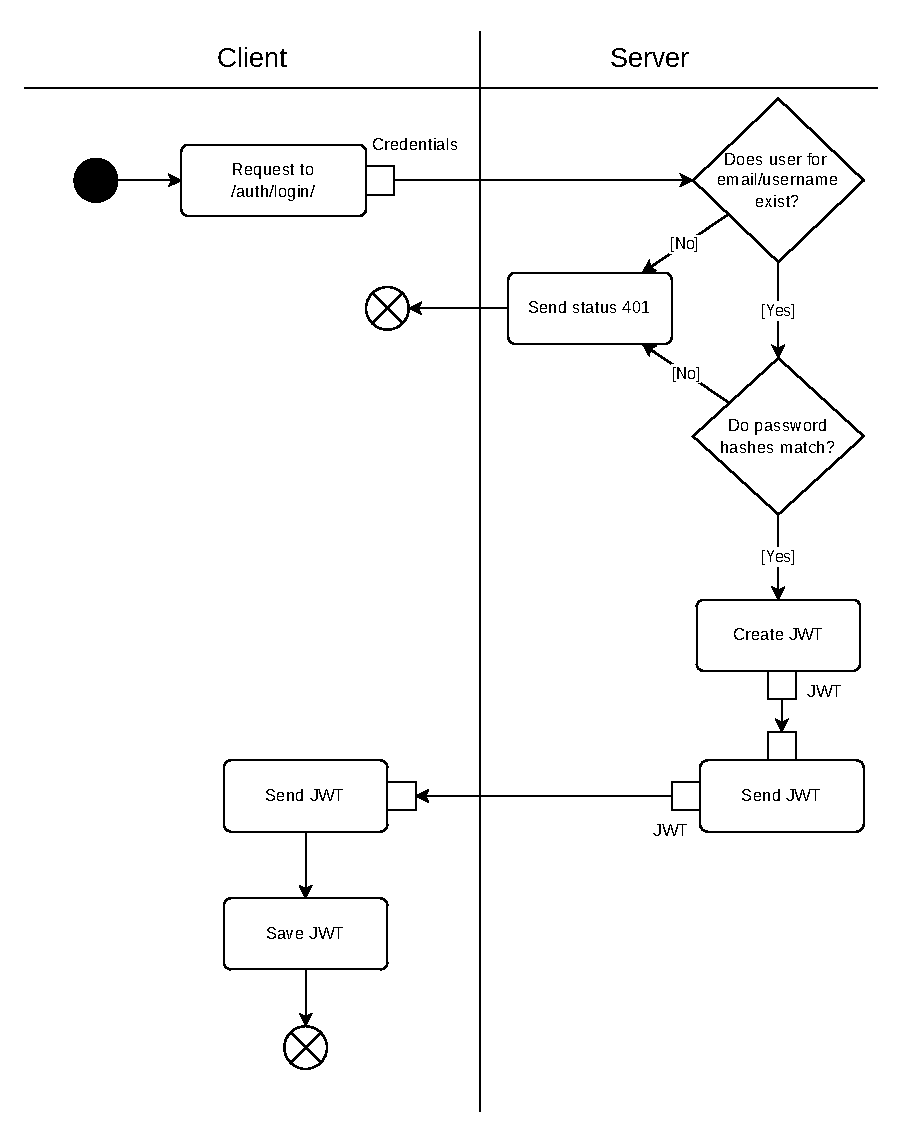
\includegraphics[width=\linewidth]{logging-in}}

    \caption{Flow for logging in}
    \label{fig:logging-in}
\end{figure}

\paragraph{Using an access-token}
When a client wants to perform a request to an endpoint that requires authentication, the \textit{JWT} is included as the value of the \textit{Bearer} header.
Before the requested action is performed, the server checks whether the JWT is valid and non-expired.
If all checks succeed, the action is performed.
If one of the checks fail, status code \textit{401} or \textit{403} is returned. \newline
Figure~\ref{fig:using-access-token} visualizes this flow.

\begin{figure}
    \centering
    \fbox{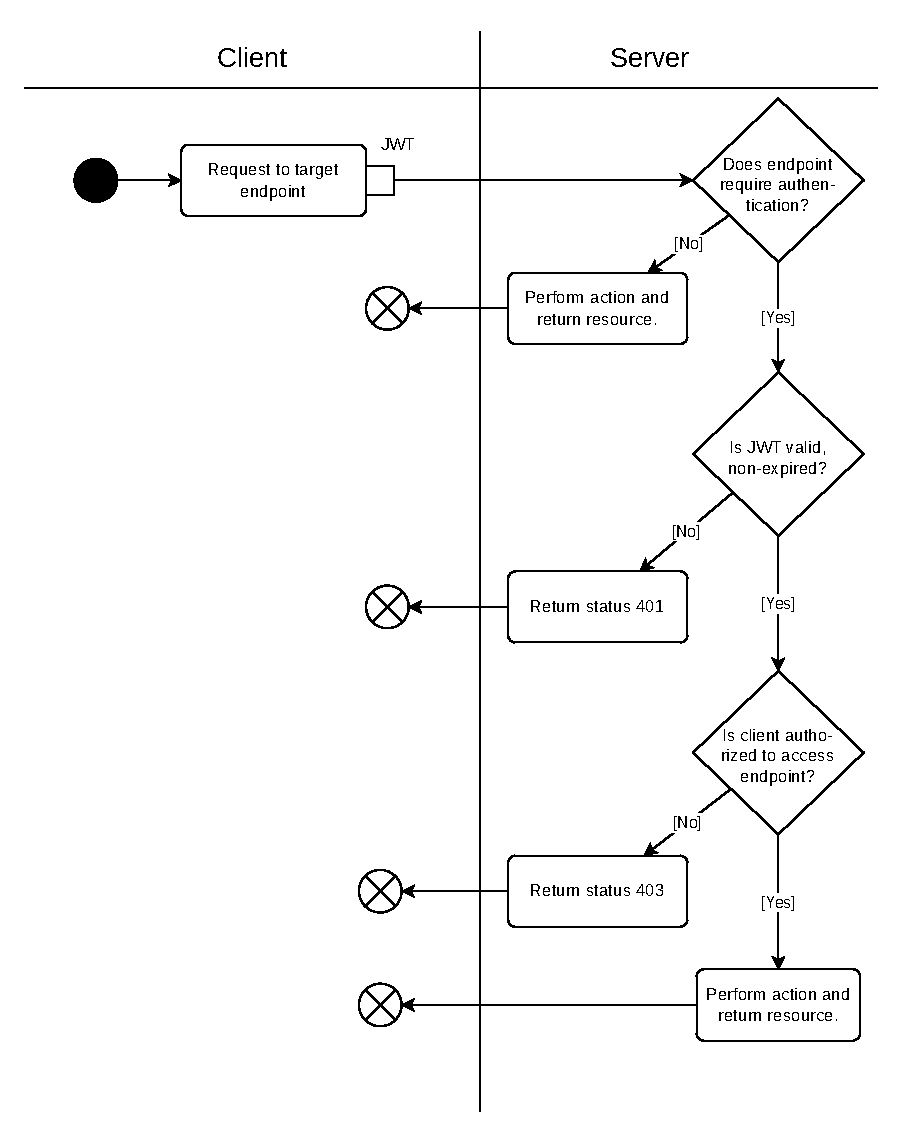
\includegraphics[width=\linewidth]{using-access-token}}

    \caption{Flow for accesing a restricted endpoint}
    \label{fig:using-access-token}
\end{figure}

\paragraph{Using a refresh-token}
When a client wants to create a new access-token using an existing refresh-token, it makes a request to \texttt{/auth/refresh/}.
The server receives the refresh-token and checks whether it exists, is non-expired and non-invalidated.
If all checks succeed, a new refresh-token is created and the old one invalidated.
Together with the new refresh-token, a new access-token is generated and returned.
If one of the checks fail, status \textit{401} is sent. \newline
Figure~\ref{fig:using-refresh-token} visualizes this flow.

\begin{figure}
    \centering
    \fbox{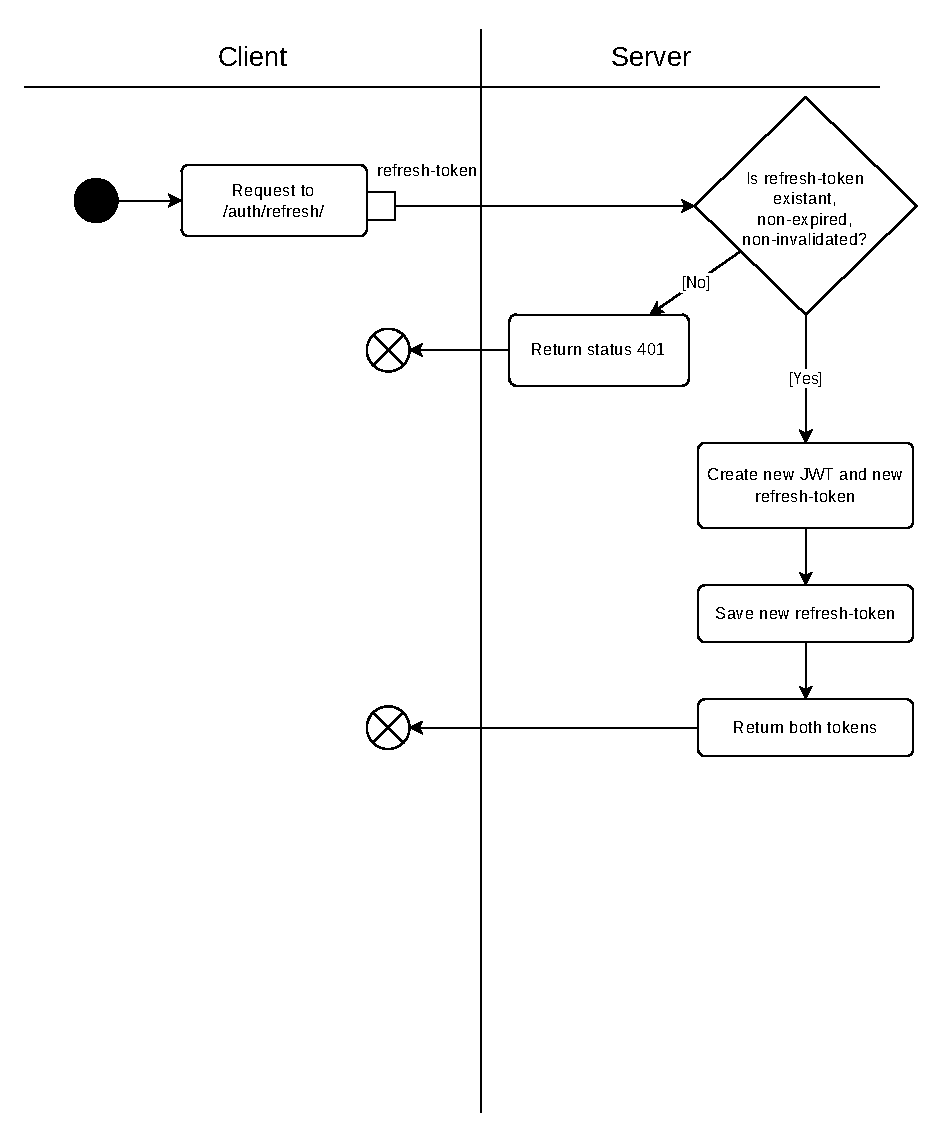
\includegraphics[width=\linewidth]{using-refresh-token}}

    \caption{Flow for refreshing}
    \label{fig:using-refresh-token}
\end{figure}

\subsection{Server fine design}\label{subsec:server-fine-design}

\subsubsection{Internal server interfaces}
In the following, we will present the fine design of the internal server interfaces, as described in~\ref{subsec:internal-server-interfaces}.

\paragraph{Request Executors}
A request executor contains multiple methods, where each method corresponds to exactly one http-method on a specific endpoint.
The method parameters are either request bodies, query parameters or path variables.
The method return values are the response bodies.\newline
The responsibility of the request executors is to ensure authorization by using the authorizer, handling errors that might occur in the services, and converting the results of the services to the response bodies.
Figure~\ref{fig:inter-executors} gives an overview over all request-executors and their methods.

\begin{figure}
    \centering
    \fbox{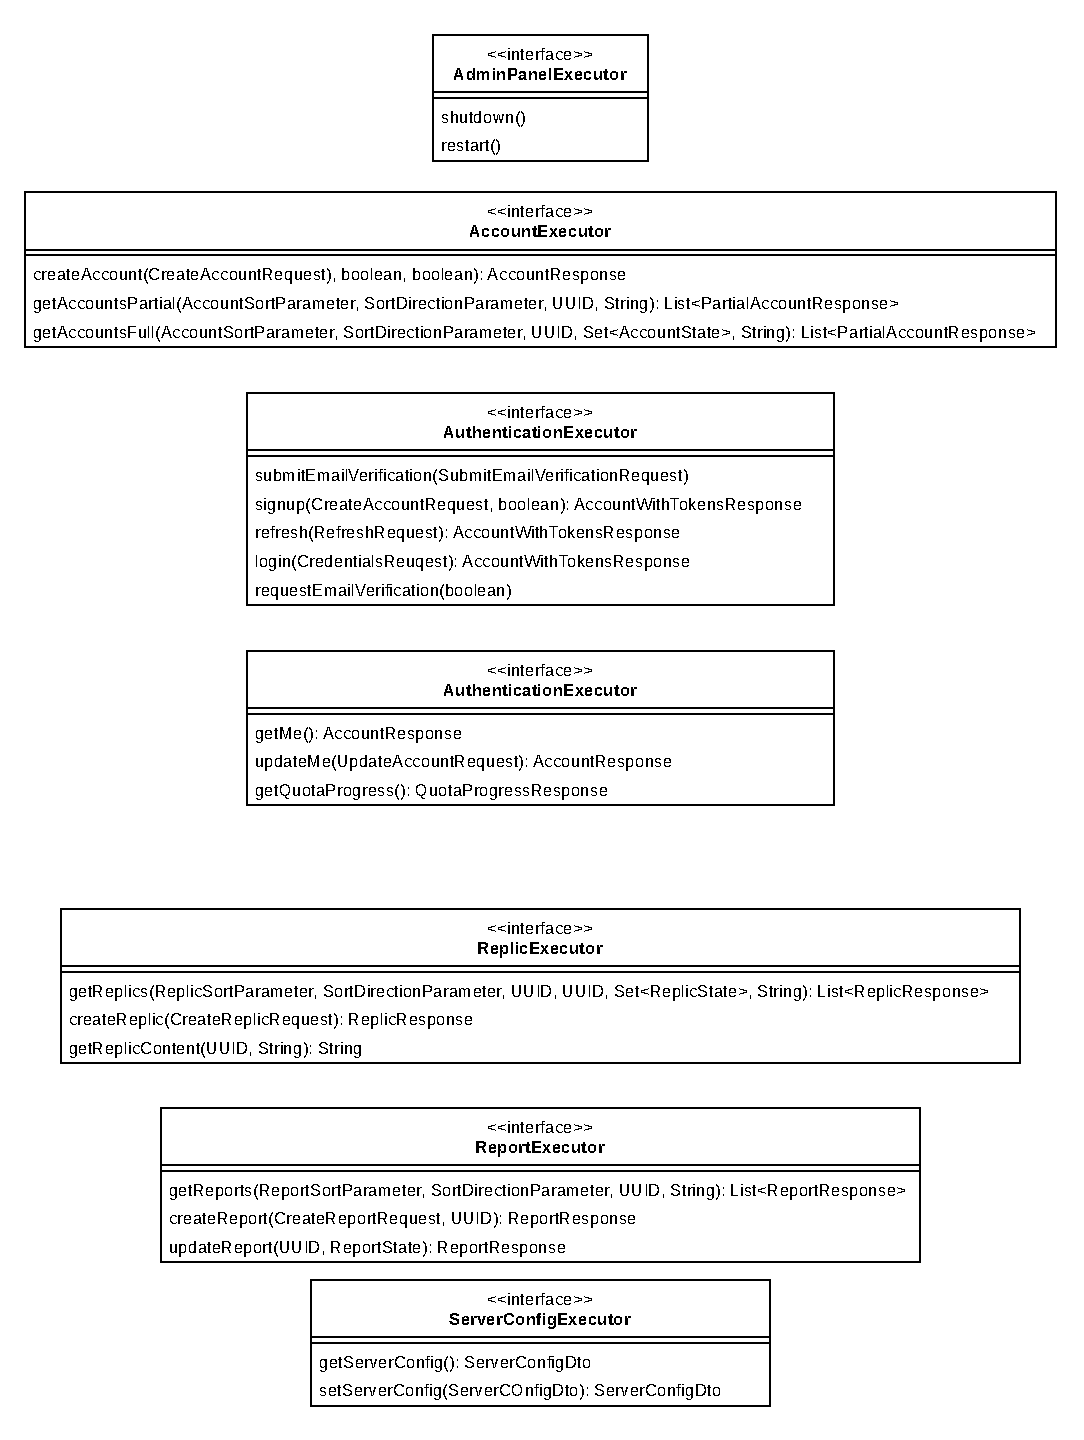
\includegraphics[width=\linewidth]{inter-executors}}

    \caption{Request Executors}
    \label{fig:inter-executors}
\end{figure}

\paragraph{Authorizer}
The authorizer makes the decisions for whether a client, authenticated or anonymous, is allowed to perform a speciifc request. \newline
In most cases, this comes down to checking whether a client fulfills the auth group set by the config, or whether the client itself is an admin.
Figure~\ref{fig:inter-authorizer} shows the methods of the authorizer interface.

\begin{figure}
    \centering
    \fbox{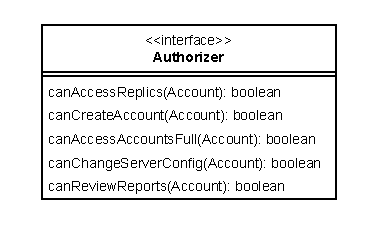
\includegraphics{inter-authorizer}}

    \caption{Authorizer}
    \label{fig:inter-authorizer}
\end{figure}

\paragraph{Domain Models}
The domain models are the basic data classes that model the business structure. \newline
They are implemented as simple java classes without further logic.
Figure~\ref{fig:domain-models} shows these classes.

\begin{figure}
    \centering
    \fbox{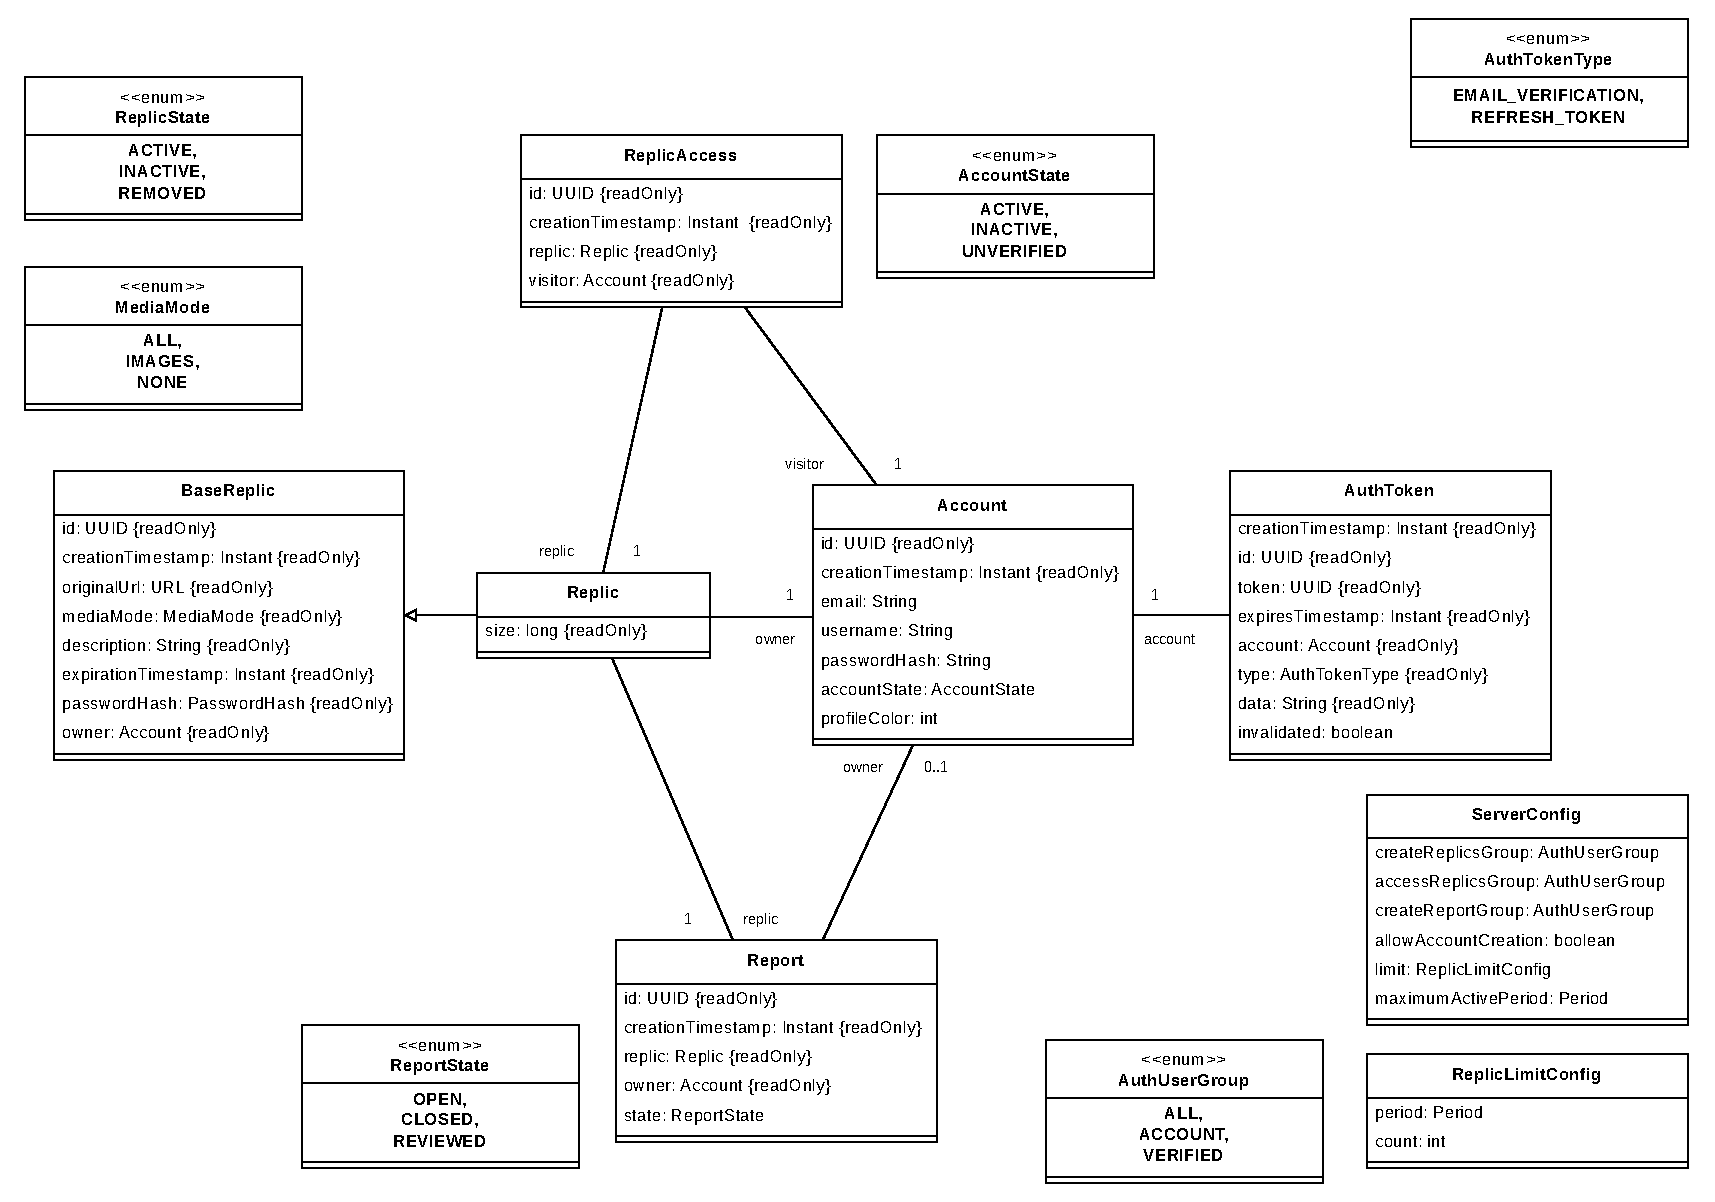
\includegraphics[width=\linewidth]{domain-models}}

    \caption{Domain models}
    \label{fig:domain-models}
\end{figure}

\paragraph{Domain Services}
The domain services encapsulate the general logic of the app. \newline
The methods of the services are held simple to keep the spirit of the domain.
To prevent returning complex result types, errors are raised by throwing checked exceptions.
Every specific type of failure has a custom exception type that is explicitly declared on the method to allow targeted handling.
Figure~\ref{fig:domain-services} shows the services and their methods.

\begin{figure}
    \centering
    \fbox{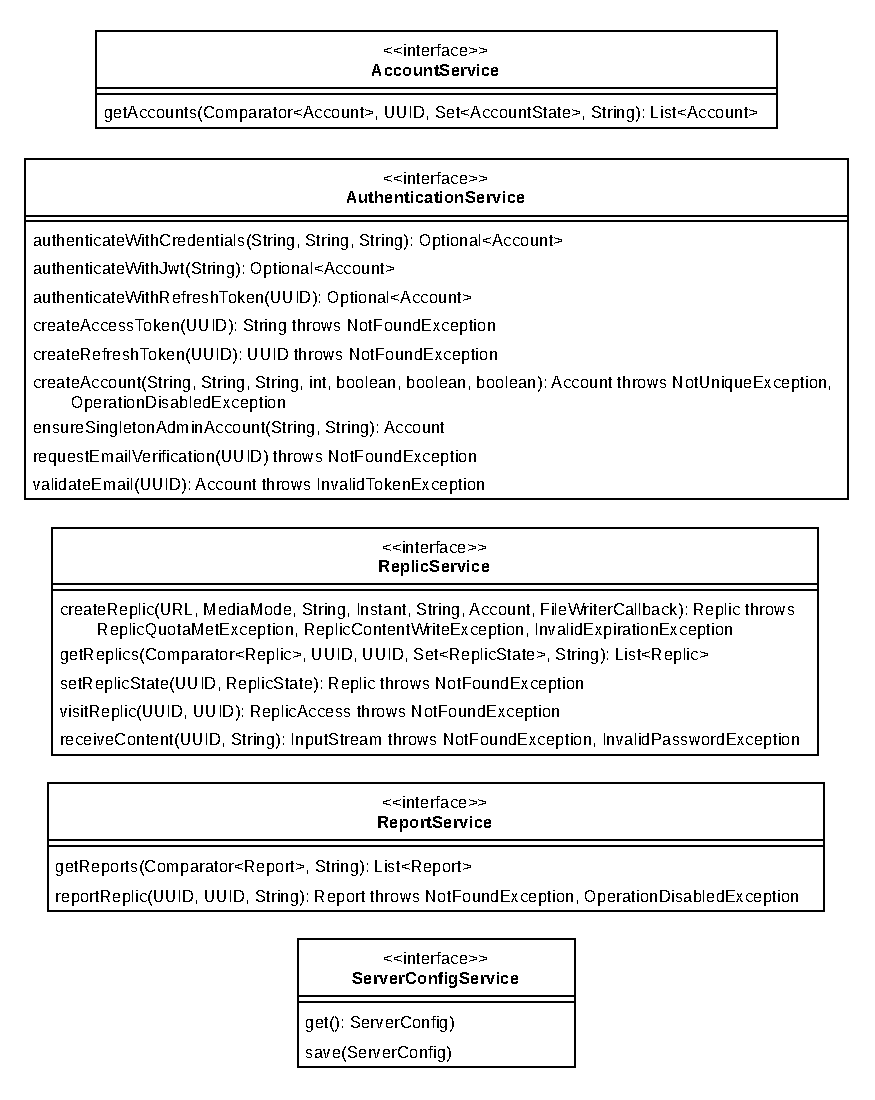
\includegraphics[width=\linewidth]{domain-services}}

    \caption{Domain services}
    \label{fig:domain-services}
\end{figure}

\paragraph{Domain repositories}
The domain repositories are the way the domain communictaes with the database. \newline
Repositories are meant to be a simple interface to queries into a specific table of the relational database.
For most models, it is sufficient to provide the simple methods \texttt{getAll}, \texttt{getById} and \texttt{save}.
Filtering logic is made by the corresponding service.
Figure~\ref{fig:domain-repositories} shows the repository-structure.

\begin{figure}
    \centering
    \fbox{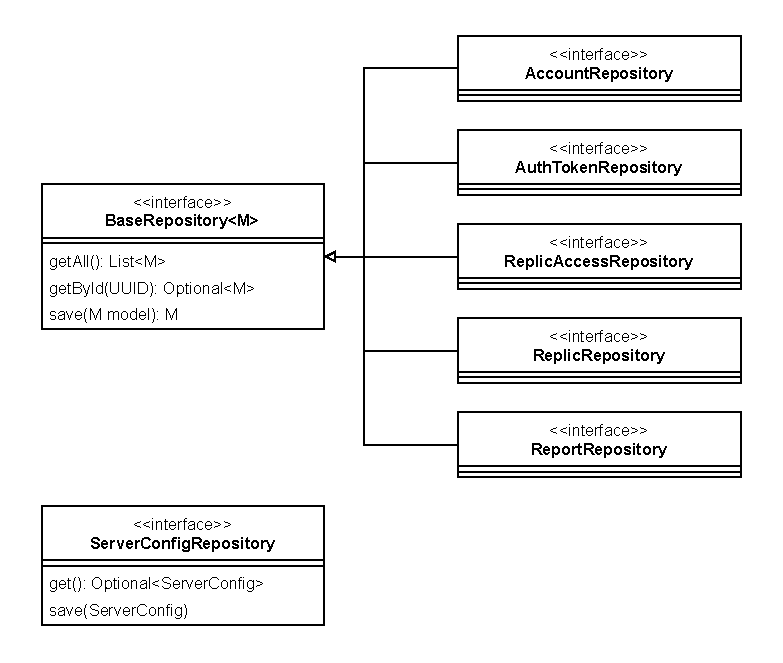
\includegraphics[width=\linewidth]{domain-repositories}}

    \caption{Domain repositories}
    \label{fig:domain-repositories}
\end{figure}

\subsubsection{Internal client interfaces: Common}
\paragraph{Network Interface}
The Network Interface provides access to the REST-API to the rest of the common model. \newline
The RestApi contains for each endpoint and http-method one method that has as its parameters the request body, query parameters and path variables, and as the return value an \texttt{Observable<T>}, where \texttt{T} is the DTO of the response body.
Figure~\ref{fig:common-networkinterface} shows the class-diagram for the RestApi.

\begin{figure}
    \centering
    \fbox{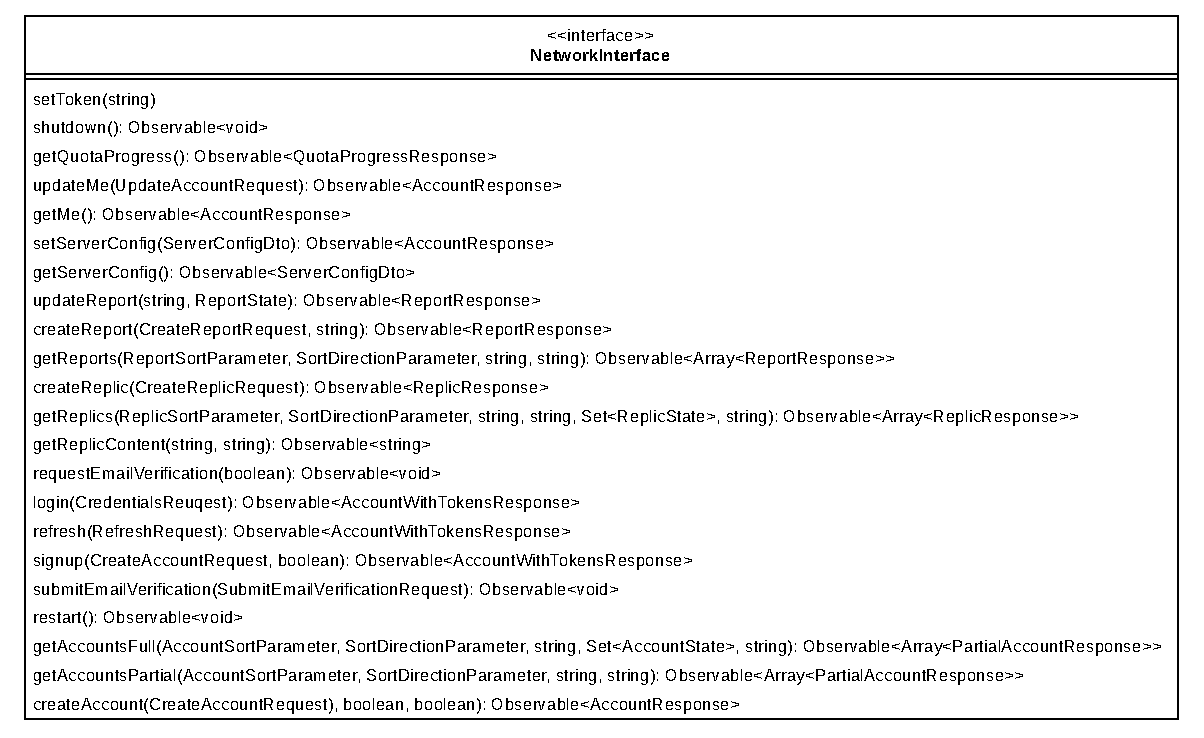
\includegraphics[width=\linewidth]{common-networkinterface}}

    \caption{Network Interface}
    \label{fig:common-networkinterface}
\end{figure}